%----------------------------------------------------------------------------------------
%	LEADERBOARD
%----------------------------------------------------------------------------------------
The leaderboard was implemented through the use of data structures that can represent the tables shown below. \textbf{Username} is an unique id on the \textit{User Records} table but not on \textit{Games Won}.
\\
\\
User Records: 
\begin{tabular}{|c|c|c|}
	\hline
	\textbf{Username}&Games Won&Games Played\\
	\hline
\end{tabular}
\quad
Games Won: 
\begin{tabular}{|c|c|}
	\hline
	\textbf{Username}&Time Taken\\
	\hline
\end{tabular}
\\
\\
When a client requests the leaderboard, the \textit{Games Won} table will be printed to the terminal. User information (games played/won) will be added to each row by getting the data from the \textit{User Records} table that matches the \textbf{Username}. 
\\
The \textit{User Records} table was implemented as a Linked List with nodes consisting of \textit{user} structures. A HEAD and a TAIL pointer were created in order to access the list. 
\begin{lstlisting}[style=CStyle]
// leaderboard.h: Lines 11-16
struct user {
	char* username;         
	int games_won;
	int games_played;     
	struct user* next; // Pointer to the next user
};

// leaderboard.c: Lines 12-13
struct user* head_userinfo = NULL;   // HEAD of the linked list of the user details
struct user* tail_userinfo = NULL;   // TAIL of the linked list of the user details
\end{lstlisting}
The \textit{Games Won} table was also implemented as a Linked List but used nodes consisting of \textit{game} structures.
\begin{lstlisting}[style=CStyle]
// leaderboard.h: Lines 22-26
	struct game {
	char* username; 
	int time_taken;       
	struct game* next;   // Pointer to the next game completed
};

// leaderboard.c: Lines 15-16
struct game* head_gameinfo = NULL;   // HEAD of the linked list of the queue of clients
struct game* tail_gameinfo = NULL;   // TAIL of the linked list of the queue of clients
\end{lstlisting}
In order to choose the data structure that will be used to represent the leaderboard, the required operations to be completed on the structure were first written down. 
\\
The most common operation will be \textit{search} followed by \textit{insert}. In some cases \textit{access} might be used and there is also no need to have functionality for a \textit{delete} operation. 
\\
Several data structures were considered and their time complexities for the required operations were written down.
\begin{center}
\begin{tabular}{|c|c|c|c|c|c|c|}
	\cline{1-7}
	& \multicolumn{3}{|c|}{Average} & \multicolumn{3}{|c|}{Worst Case}	\\
	\cline{1-7}
	Data Structure & Search & Insertion & Access & Search & Insertion & Access \\
	\hline
	Array				& O(n)	& O(n)	& O(1)	& O(n)	& O(n)	& O(1)	\\
	Singly-Linked List	& O(n)	& O(1)	& O(n)	& O(n)	& O(1)	& O(n)	\\
	Hash Table			& O(1)	& O(1)	& N/A	& O(n)	& O(n)	& N/A	\\
	Red-Black Tree		& O(logn) & O(logn) & O(logn) & O(logn) & O(logn) & O(logn) \\
	\hline
\end{tabular}
\end{center}
Initally, a Red-Black tree was going to be used. However, the extra complexity it would add for a programmer to read/debug and the extra time it would take to implement is not worth the small gains in computational efficiency. 
\\ 
As the leaderboard is wiped whenever the server shuts down, \textit{n} has a low chance of reaching a large enough value where the extra efficiency from a Red-Black Tree will be felt.
\\
A Singly-Linked List was chosen in the end as it is the simplest data structure that could've been implemented (as a Linked List was already in use for the client queue) while providing good efficiency for the most used operations. 
\begin{figure} [!ht]
	\centering
	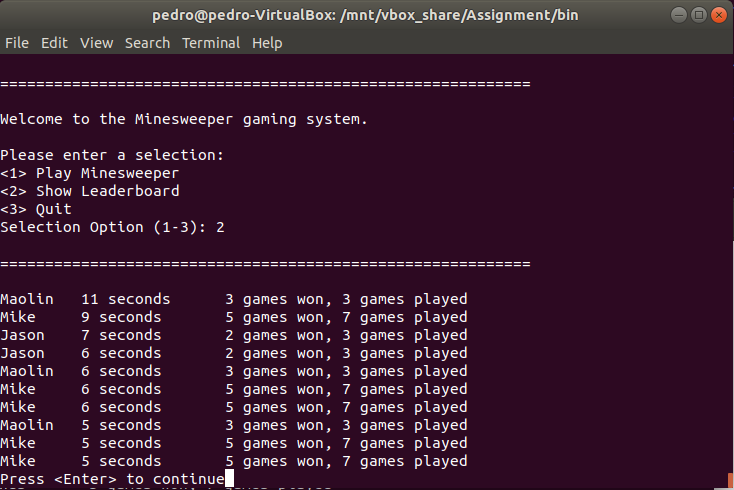
\includegraphics[width=1\textwidth]{images/Leaderboard} 
	\caption{The leaderboard with examples of how it is sorted and displayed}
	\label{fig:leaderboard} 
\end{figure}